% !TeX root = ../main.tex

\chapter{面向近存架构的高效算法设计}


\section{概述}\label{sec:nmp-overview}
现有的最佳优先搜索算法在冯诺依曼架构上执行非常低效,原因是搜索算法主要的算子之一是距离计算。
计算两个向量之间的距离,由于图算法的特性,导致向量数据对于某个查询来说不存在复用,因此整个搜索算法的76.7\%的时间开销在访存上

近邻图搜索算法的算子有以下几种,分别是:距离计算、过滤、排序和索引。


\section{方法介绍}\label{sec:nmp-method}
在本节中会重点介绍本章所提出的面向近存架构的高效算法设计方法。首先介绍近邻图搜索算法的建模,指出在CPU上的距离计算操作是整个搜索算法的瓶颈。然后在\ref{sec:nmp-method-distance}节中介绍搜索算法中距离计算操作并行化的方法。当距离计算操作被并行化后,排序操作会成为限制性能进一步提升的瓶颈。最后在\ref{sec:nmp-method-sort}节介绍延迟排序策略,以实现搜索算法在近存架构上的完全流水(图~\ref{fig:software-opt}(e))。

\begin{figure}[htbp]
  \centering
  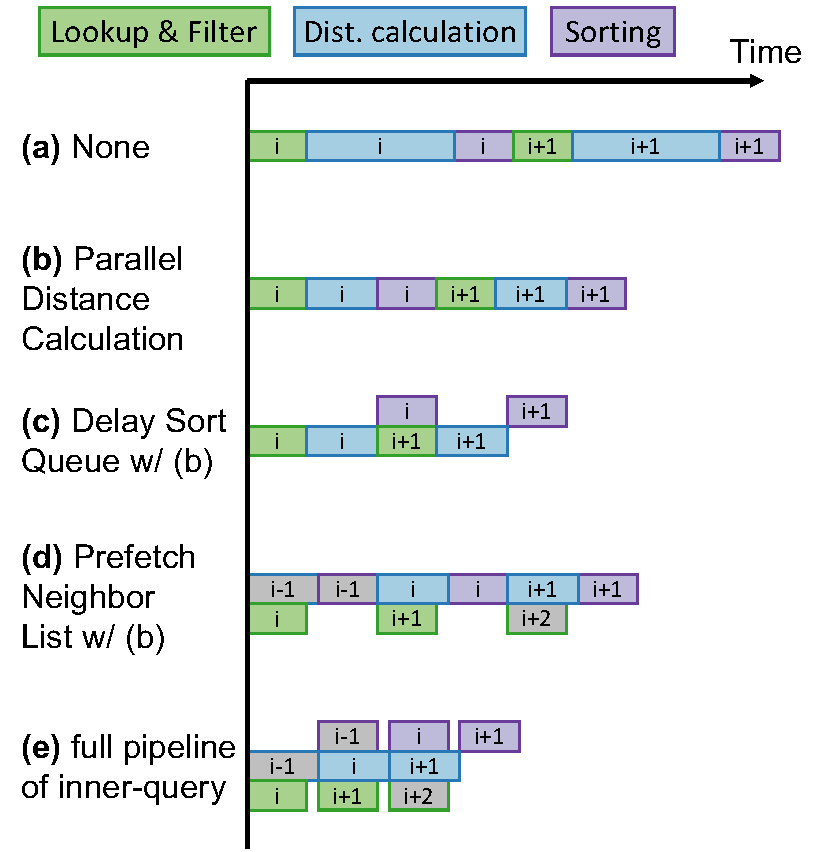
\includegraphics[width=0.45\textwidth]{figures/context-2/software-opt.pdf}
  \caption{Software solutions. \todo{Add figures}}
  \label{fig:software-opt}
\end{figure}

\subsection{近邻图搜索算法建模}\label{sec:nmp-method-model}
% 针对单机的搜索算法建模
% 合并一下我之前的模型(简化一些)+华哥列的计算表达式,突出体现有几个计算步骤,承接下面的两个技术
本节对近邻图搜索算法进行建模和分析。如前所述,对于某个查询点,它完整的搜索过程是由若干个轮次组成的,总轮次记为$\#round$。那么,整个近邻图搜索算法的执行时间可以表示为:
\begin{equation}
  T_{query}=\#iter\times \left( T_{nlist}+T_{filter}+T_{dist}+T_{sort} \right)
  \label{eq:nmp-overall}
\end{equation}

整个搜索过程包括以下四个算子:
\begin{enumerate}
  \item \textbf{取邻居列表}~根据当前搜索点,获取它的全部邻居;
  \item \textbf{过滤重复点}~由于部分邻居点已经在之前的轮次中被计算过和查询点之间的距离,为了避免重复计算,需要将这些计算过的邻居点去掉;
  \item \textbf{距离计算}~对于过滤后的邻居点,逐个计算它们和查询点之间的距离;
  \item \textbf{排序}~将本轮完成计算的邻居点,根据它们与查询点的距离,逐个添加到搜索队列中。
\end{enumerate}

相应的,

式~\ref{eq:nmp-overall}中的$T_{nlist}$表示取邻居列表的执行时间,可进一步表示为:
\begin{equation}
  T_{nlist}=\#nbor\times l_{index}\times t_{mem}
\end{equation}
其中$\#nbor$表示搜索点的邻居数量(下同),$l_{index}$表示每个邻居点所需要的存储量(例如,4字节),$t_{mem}$表示获取单位数据用于计算所需要的时间开销(下同),这一时间与实际的硬件实现方式有关。

式~\ref{eq:nmp-overall}中的$T_{filter}$表示过滤重复点的执行时间,可进一步表示为:
\begin{equation}
  T_{filter}=\#nbor\times t_{filter}
\end{equation}
其中$t_{filter}$表示过滤一个邻居点所需要的时间开销,这一时间与实际硬件和实现方式都有关,例如在CPU上可以通过查表的方式实现。

式~\ref{eq:nmp-overall}中的$T_{dist}$表示距离计算的执行时间,可进一步表示为:
\begin{equation}
  T_{dist}=\#nbor\prime \times \left(\#dim\times l_{value}\times t_{mem} + t_{calc} \right)
\end{equation}
其中$\#nbor\prime$表示搜索点过滤后的邻居数量(下同),一般与$\#nbor$相差不大,实验中平均有10\%-20\%的点会被过滤掉。$\#dim$表示数据点特征的维度,$l_{value}$表示每个维度数据所需要的存储量(例如常见的有,1字节的$int8$和$uint8$数据类型,4字节的$float32$数据类型)。$t_{mem}$的含义同上,$t_{calc}$表示计算单个点与查询距离的时间开销。由于查询点的数据是频繁被使用的,因此距离计算操作只考虑了一个向量的访存情况。

式~\ref{eq:nmp-overall}中的$T_{sort}$表示排序的执行时间,可进一步表示为:
\begin{equation}
  T_{sort}=\#nbor\prime \times t_{sort}
\end{equation}
其中$t_{sort}$表示将一个点插入到优先队列中所需要的时间开销。

基于上述的分析,本文进一步对HNSW近邻图搜索算法在CPU上的时间开销组成进行了分析。本文分别在SIFT10M和DEEP10M两个数据集上进行了测试,结果如图~\ref{fig:operation-time}所示。可以发现,距离计算是整个搜索过程中时间开销占比最大的操作,占比高达85\%以上,其次是排序操作占比在10\%左右,重复点过滤占比在5\%左右。由于取邻居列表的时间开销很小,因此归类到其他中。

\begin{figure}
  \centering
  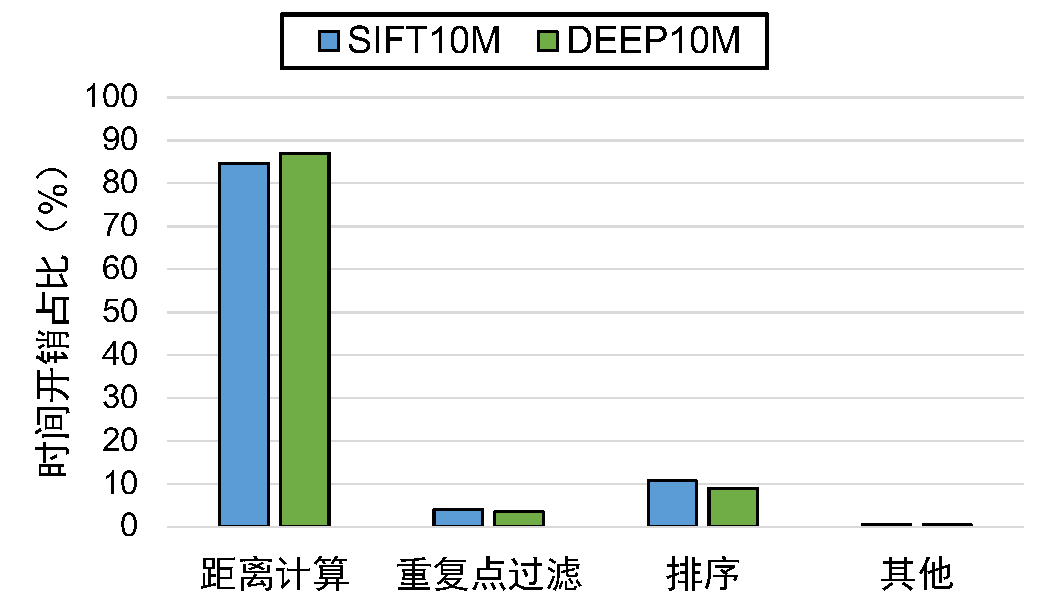
\includegraphics[width=0.6\textwidth]{figures/context-2/operation-time.pdf}
  \caption{每个操作在CPU上运行的时间开销百分比}
  \label{fig:operation-time}
\end{figure}


\subsection{面向近存的并行算法设计}\label{sec:nmp-method-distance}
% 不同的分配方法,以及过滤操作也要并行?
综上所述,近邻图搜索算法中的距离计算操作是整个计算过程的瓶颈。根据\ref{sec:nmp-method-model}节的建模不难发现,这一挑战的原因有两个:一方面,距离计算操作需要读取数据特征,因此访存量是其他操作的几十倍(例如SIFT数据集,对于某个点来说,其特征大小为128维度\times1字节,而索引大小仅为4字节;DEEP数据集单个点的特征大小为96维度\times4字节)。另一方面,搜索是根据近邻图进行的,而图这种数据结构具有天然的不规则访存的特点。上述两个问题叠加在一起,导致了近邻图搜索算法在现有冯诺依曼架构上的低效。因此,本文采用近存架构来解决这一问题。

% TODO:背景或者基础部分需要介绍一下DRAM?
为了充分发挥近存架构的潜在能力,需要设计高效的算法,将近邻图搜索映射在近存架构上。其中距离计算和重复点过滤两个操作比较容易实现并行化,因此将它们通过并行的方式在近存架构的rank层级上执行。整个图的特征是以矩阵的方式紧密存储的(即,特征矩阵),矩阵的行数就是图上的点数,矩阵的列数是数据特征的维度。因此需要将特征矩阵分成$N_r$个部分($N_r$是可供使用的rank数量,因为索引矩阵也需要一定的存储空间),以并行的方式执行距离计算操作。并行化距离计算操作的实际执行时间依赖于$N_r$中执行时间最长的那个,因此我们需要选择一个更好的映射方法(特征矩阵到子特征矩阵)。测试了两种典型的映射方法:顺序映射和模映射。顺序映射是将特征矩阵依次划分为$N_r$子特征矩阵。模映射是将特征矩阵的基向量依次划分为不同的子特征矩阵。Eq. \ref{eq:mapping}给出了这两种映射方法的计算表达式。
\begin{equation}\label{eq:mapping}
\begin{split}
L_{seq}\left(Id\right) = Id / \left \lceil N / N_r \right \rceil \\
L_{mod}\left(Id\right) = Id\ mod\ N_r
\end{split}
\end{equation}

首先分析了这两种映射方法的理论性能;如图\ref{fig:parallel-dist}(左)所示,其中$N_r=4$,由于总的计算量相同,利用率最低的子特征矩阵决定了最终距离计算的性能。与串行映射相比,模映射的性能提高了27\%。此外,我们还分析了加速比与$N_r$的关系,我们发现当$N_r=4$时,并行距离计算可以达到2.7倍的加速比(图\ref{fig:parallel-dist}(右))。因此,可以通过模映射实现距离计算的并行化。

\begin{figure}
  \centering
  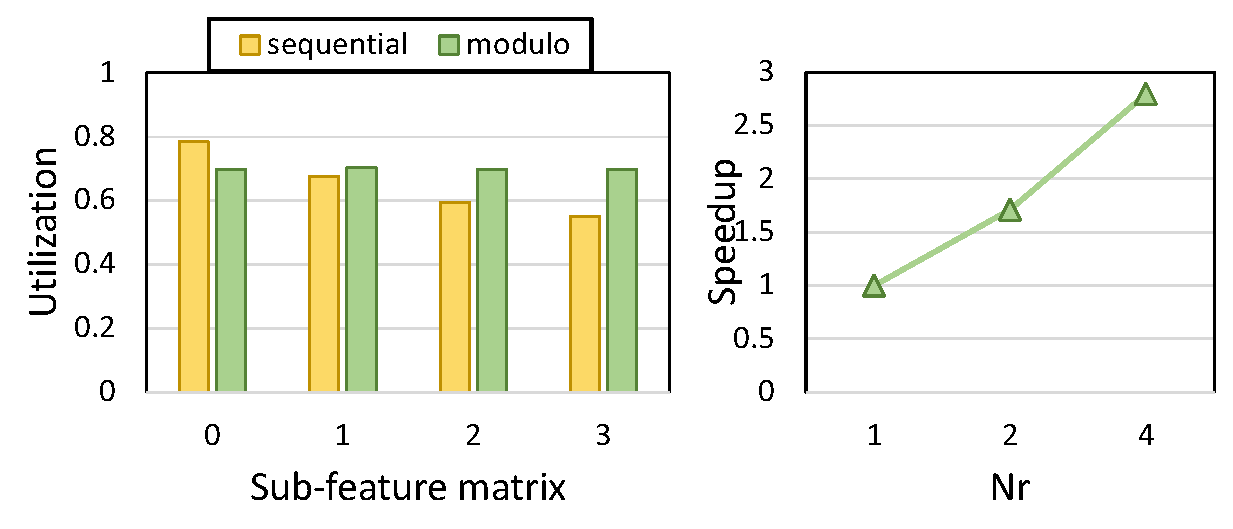
\includegraphics[width=0.9\textwidth]{figures/context-2/parallel-dist.pdf}
  \caption{左:子特征矩阵的利用率分布,最终性能取决于利用率最差的子特征矩阵。右:使用模映射方法加速比和$N_r$之间的关系。}
  \label{fig:parallel-dist}
\end{figure}

\subsection{延迟排序方法}\label{sec:nmp-method-sort}
距离计算操作并行化后,排序的时间开销不可忽视。为此,提出延迟排序队列策略来隐藏排序的时间开销。在原始的搜索算法计算流程中,$i$ -th步搜索依赖于$(i-1)$ -th排序结果,导致排序操作不能与其他操作并行执行。
经过分析,我们发现$i$-th步骤的搜索点($i>1$)只有两个来源。一个是$(i-1)$ -th步骤中最近的未搜索点,另一个是$(i-1)$ -th步骤距离计算结果中最小$Dist.$的点($Id_{dcmin}$)。根据这个特性,我们可以在距离计算操作之后无需排序操作就可以开始下一步的搜索。

我们需要添加两个更改来实现这个策略。(1)在距离计算操作中,每个子特征矩阵需要额外输出一个最小的点$Dist.$,并选择最小的点作为$Id_{dcmin}$。(2)在选择操作中,$i$ -th步骤中的搜索点只需选择$(i-2)$ -th步骤中的最近未搜索点与$(i-1)$ -th步骤中的$Id_{dcmin}$之间距离最小的搜索点。
然后,我们分析了延迟排序队列策略带来的额外开销,与并行距离计算方法相比,它仅占总运行时间的0.5\%。




\section{实验结果}\label{sec:nmp-experiment}
\subsection{实验设置}

\subsection{实现方法}
% 在FPGA上进行了验证

\subsection{整体性能}

\subsection{消融实验}




\section{本章小结}\label{sec:nmp-conclusion}


